\documentclass[12pt]{article}

\setlength{\topmargin}{-.75in} \addtolength{\textheight}{2.00in}
\setlength{\oddsidemargin}{.00in} \addtolength{\textwidth}{.75in}

\usepackage{amsmath,color,graphicx,array,multirow,rotating, enumerate}
\usepackage{type1cm}
\usepackage{eso-pic}
\usepackage[hmargin=2cm,vmargin=1.3cm]{geometry}
\usepackage{mathabx}
\usepackage[rflt]{/Users/jgates/desktop/latex/floatflt}
\usepackage[table]{xcolor}
\nofiles

\def\Tab#1{\tabular[t]{>{\rule[-1ex]{0pt}{3ex}}c}#1\endtabular}
\newcolumntype{C}{@{}c@{}}

\pagestyle{empty}
\newcounter{ProbNum}
\setlength{\parindent}{0in}

% Watermark: graph paper
\newcommand\BackgroundPic{
\put(0,0){
\parbox[b][\paperheight]{\paperwidth}{%
\vfill
\centering

\includegraphics[width=\paperwidth,height=\paperheight,keepaspectratio]{/Users/jgates/desktop/latex/pics/plain.pdf}%
\vfill
}}}

%Diagram box command [v space][content]
\newcommand{\diagrambox}[2][40 mm]{
\framebox{\parbox{175 mm}{#2 \hfill \\ \vspace{#1}}}

\bigskip
}

% MakeList: [example number] [content]
\newcommand{\MakeList}[2]{
\begin{enumerate}[#1] \itemsep1pt \parskip0pt \parsep0pt  

#2
\end{enumerate}
}

\begin{document}



{\Large Problems tagged with standards:}Units
\bigskip 
% Number 130
% CVPMA Algebra Units
% Raptor/BSG drifting apart
% JG

% Watermark
\AddToShipoutPicture*{\BackgroundPic}

\addtocounter {ProbNum} {1}

%\begin{floatingfigure}[r]{.3\textwidth}
%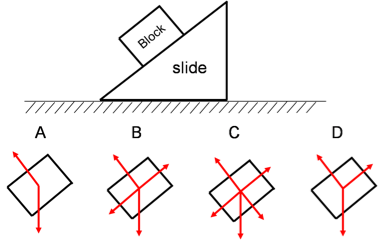
\includegraphics[scale=.4]{/Users/jgates/desktop/latex/pics/incline3.png}
%\end{floatingfigure}
 
{\bf \Large{130.}} Gaeta's Raptor is drifting away from Galactica at a speed of 200 meters per second, while the Galactica drifts away from the Raptor at a speed of 75 meters per second.  The two ships are initially 300 km away from each other.

\bigskip

\indent  How much time will pass before they are 600 km away from each other, and communication is lost?

\bigskip 
\vspace{6mm}% Number 140
% CVPMG Units
% Draw the missing graphs
% JG

% Watermark
\AddToShipoutPicture*{\BackgroundPic}

\addtocounter {ProbNum} {1}

%\begin{floatingfigure}[r]{.3\textwidth}
%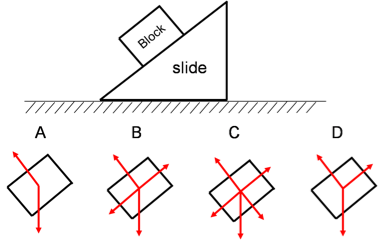
\includegraphics[scale=.4]{/Users/jgates/desktop/latex/pics/incline3.png}
%\end{floatingfigure}
 
{\bf \Large{140.}} Draw the missing graphs.

\bigskip

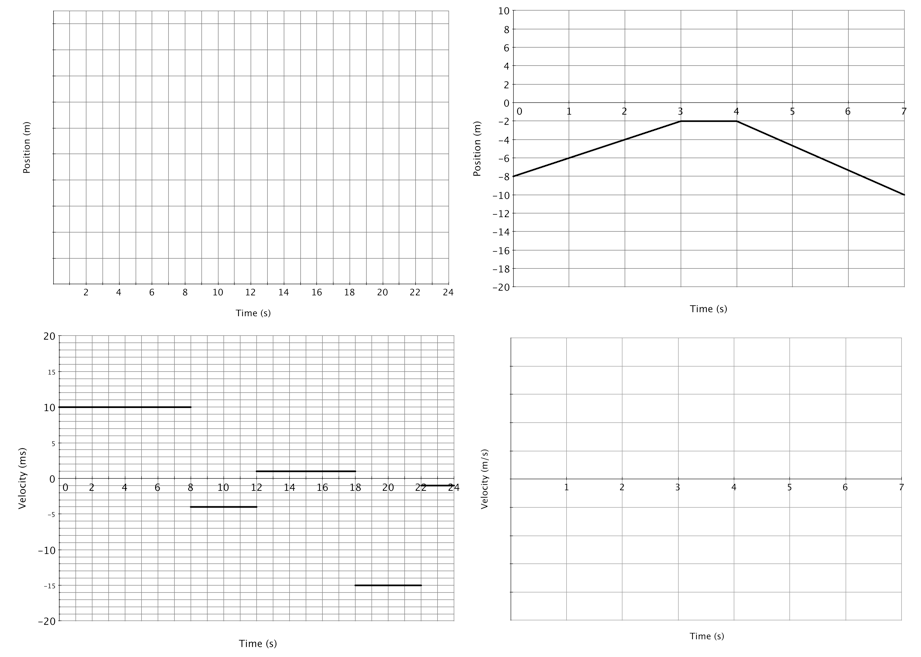
\includegraphics[scale=.57]{/Users/jgates/desktop/latex/pics/cvpmgraphs1.png}

\bigskip 
\vspace{6mm}% Number 150
% CVPMG Units
% Problem-solving, Creed and Kevin on bikes
% JG

% Watermark
\AddToShipoutPicture*{\BackgroundPic}

\addtocounter {ProbNum} {1}

%\begin{floatingfigure}[r]{.3\textwidth}
%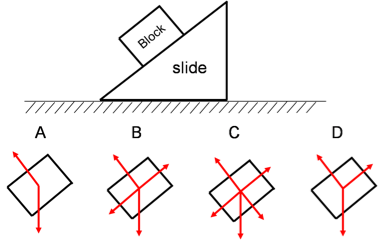
\includegraphics[scale=.4]{/Users/jgates/desktop/latex/pics/incline3.png}
%\end{floatingfigure}
 
{\bf \Large{150.}} Creed and Kevin find some bikes by the loading dock, and devise a competition: they use an 8 meter long rope to tie their bikes together and set up next to each other, facing opposite directions.  They begin next to each other, start their pedaling at the same time and ride in opposite directions, trying to see who can ride the furthest before the rope snaps tight. If Creed can pedal his bike at 4 meters per second, and he ends up 5.1 meters away from the starting point, how fast did Kevin pedal?  Solve it graphically!  Assume that they can get up to speed instantly.

%\bigskip

%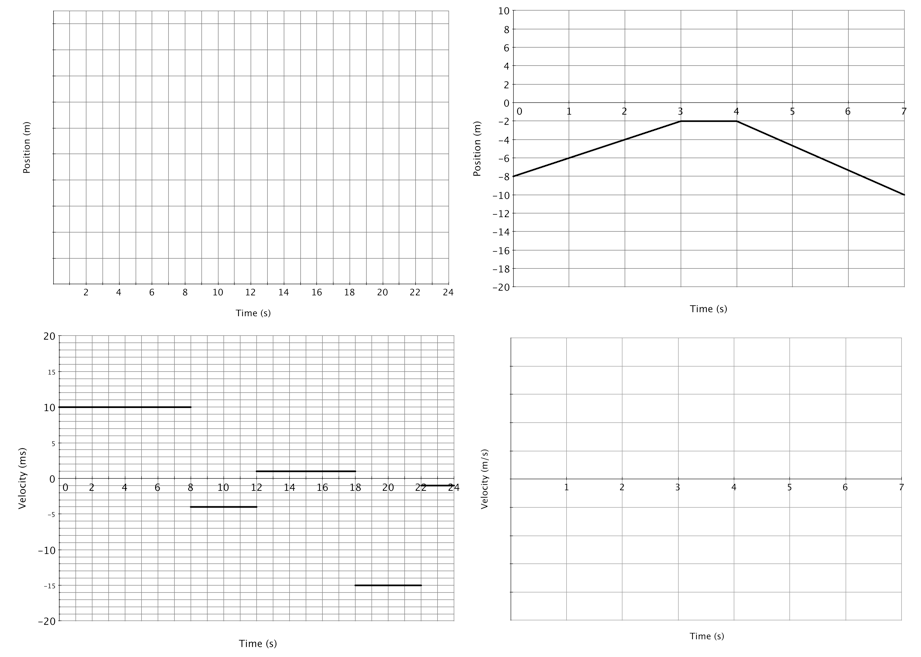
\includegraphics[scale=.57]{/Users/jgates/desktop/latex/pics/cvpmgraphs1.png}

\bigskip 
\vspace{6mm}% Number 160
% CVPMA Units Algebra Prefixes
% Problem-solving, Nostromo signal - hard!
% JG

% Watermark
\AddToShipoutPicture*{\BackgroundPic}

\addtocounter {ProbNum} {1}

%\begin{floatingfigure}[r]{.3\textwidth}
%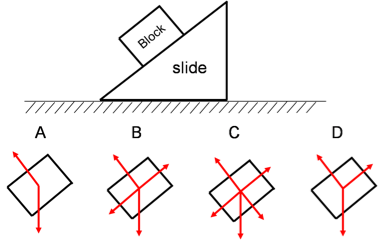
\includegraphics[scale=.4]{/Users/jgates/desktop/latex/pics/incline3.png}
%\end{floatingfigure}
 
{\bf \Large{160.}} As its crew sleeps, the Nostromo glides through space at a brisk clip of ${920~\tfrac{km}{s}}$, relative to a nearby asteroid that it is approaching.  The computer uses radar (object detection using radio waves, which travel at the speed of light: ${3 \times 10^8 ~\tfrac{m}{s}}$) to detect objects in the ship's path.  The radio waves are emitted by the ship, bounce off of the asteroid, and return to the ship, where the computer analyzes the results.

\bigskip
Assume that the asteroid begins at the limit of the ship's effective radar range of 2 million km.  Once it detects the asteroid, the computer will require 15 minutes to revive the crew.  

\bigskip

How much time will the crew have to turn the ship at that point?
%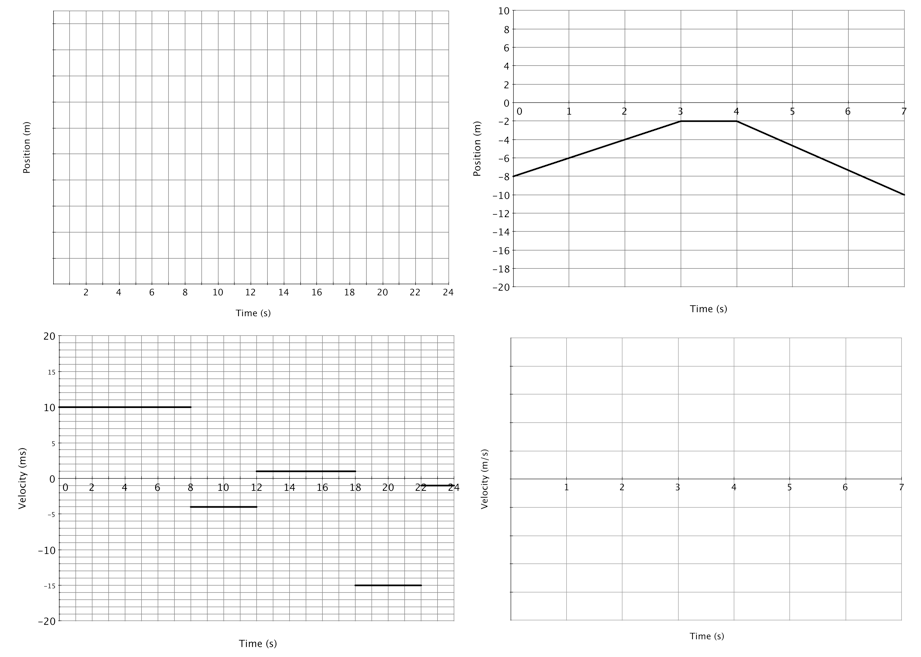
\includegraphics[scale=.57]{/Users/jgates/desktop/latex/pics/cvpmgraphs1.png}

\bigskip 
\vspace{6mm}% Number 160
% CVPMA Algebra Units Prefixes
% Problem-solving, Nostromo signal - hard!
% JG

% Watermark
\AddToShipoutPicture*{\BackgroundPic}

\addtocounter {ProbNum} {1}

%\begin{floatingfigure}[r]{.3\textwidth}
%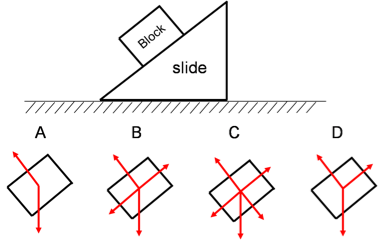
\includegraphics[scale=.4]{/Users/jgates/desktop/latex/pics/incline3.png}
%\end{floatingfigure}
 
{\bf \Large{170.}} As its crew sleeps, the Nostromo glides through space at a brisk clip of ${920~\tfrac{km}{s}}$, relative to a nearby asteroid that it is approaching.  The computer uses radar (object detection using radio waves, which travel at the speed of light: ${3 \times 10^8 ~\tfrac{m}{s}}$) to detect objects in the ship's path.  The radio waves are emitted by the ship, bounce off of the asteroid, and return to the ship, where the computer analyzes the results.

\bigskip
Assume that the asteroid begins at the limit of the ship's effective radar range of 2 million km.  Once it detects the asteroid, the computer will require 15 minutes to revive the crew.  

\bigskip

How much time will the crew have to turn the ship at that point?
%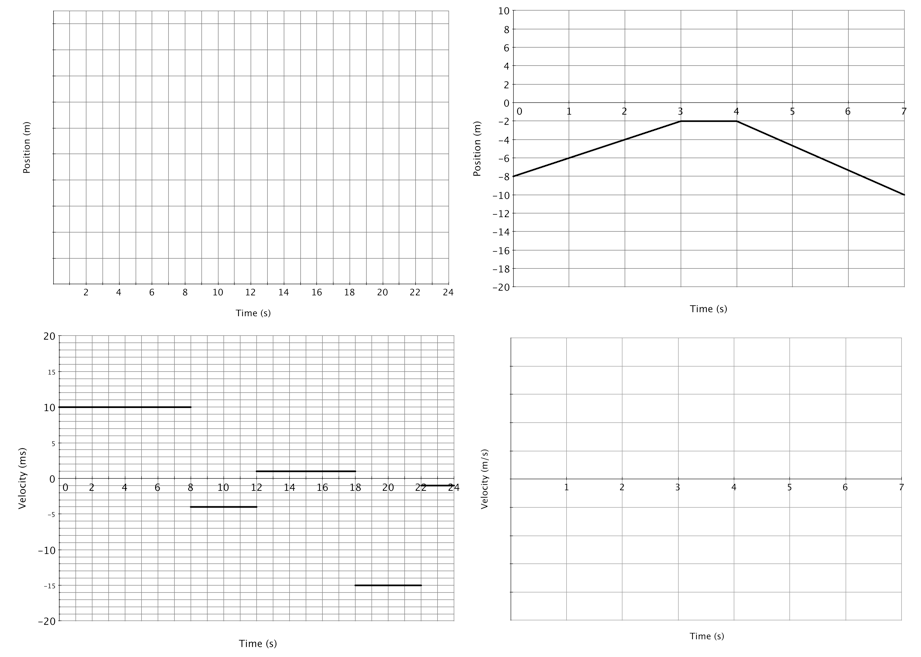
\includegraphics[scale=.57]{/Users/jgates/desktop/latex/pics/cvpmgraphs1.png}

\bigskip 
\vspace{6mm}% Number 180
% CVPMA Algebra Units 
% Problem-solving, RC cars passing each other - hardish
% JG

% Watermark
\AddToShipoutPicture*{\BackgroundPic}

\addtocounter {ProbNum} {1}

%\begin{floatingfigure}[r]{.3\textwidth}
%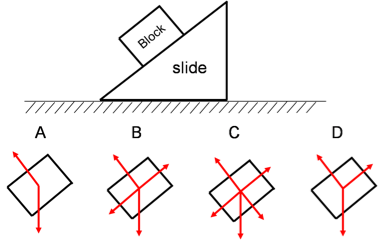
\includegraphics[scale=.4]{/Users/jgates/desktop/latex/pics/incline3.png}
%\end{floatingfigure}
 
{\bf \Large{180.}} A fast RC car (speed: ${12~\tfrac{m}{s}}$ and a slower RC car (${8~\tfrac{m}{s}}$) are 40 meters apart. They then drive directly towards each other.  Some time after the cars have passed each other, the faster car is 15 meters away from the slower one.  

\bigskip

At this moment, how far has the slower one traveled from its starting position? 

%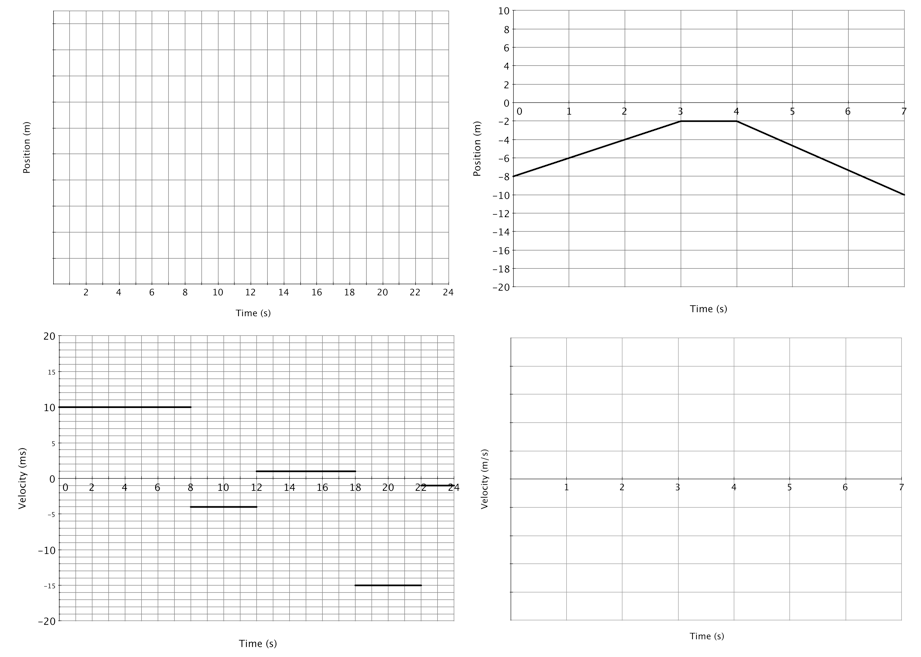
\includegraphics[scale=.57]{/Users/jgates/desktop/latex/pics/cvpmgraphs1.png}

\bigskip 
\vspace{6mm}% Number 190
% CVPMA Algebra Units OddUnits
% Problem-solving, mile marker problem
% Walker

% Watermark
\AddToShipoutPicture*{\BackgroundPic}

\addtocounter {ProbNum} {1}

%\begin{floatingfigure}[r]{.3\textwidth}
%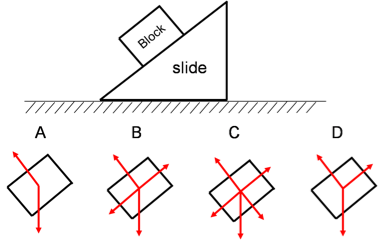
\includegraphics[scale=.4]{/Users/jgates/desktop/latex/pics/incline3.png}
%\end{floatingfigure}
 
{\bf \Large{190.}} You're driving along the highway at constant speed.  When you increase your speed by ${7.9~\tfrac{mi}{hr}}$, the time to go one mile decreases by 13 s. 

\bigskip

What was your original speed?  

%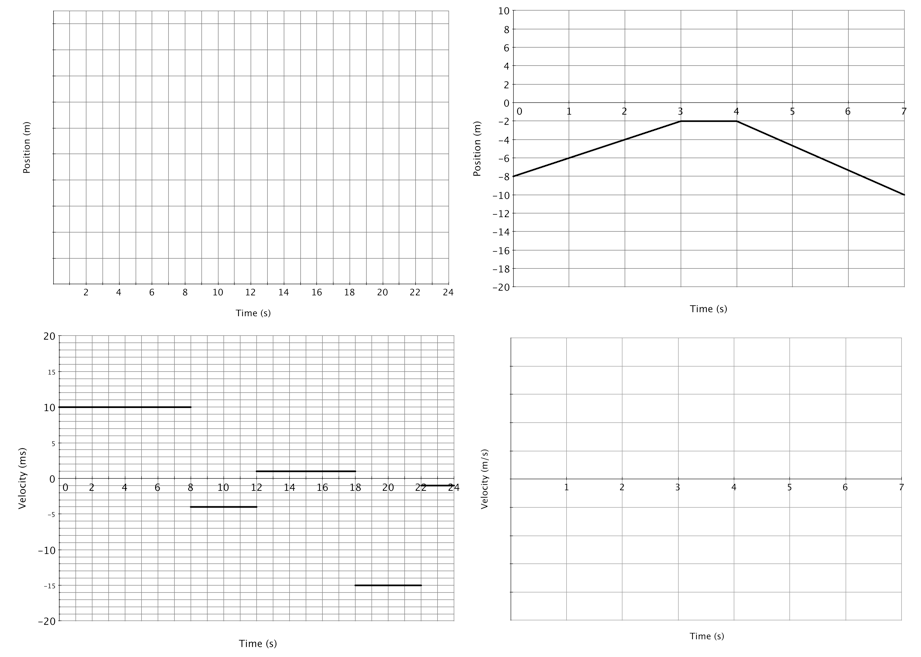
\includegraphics[scale=.57]{/Users/jgates/desktop/latex/pics/cvpmgraphs1.png}

\bigskip 
\vspace{6mm}% Number 200
% CVPMG Units
% v to x graph, quantitative
% Walker

% Watermark
\AddToShipoutPicture*{\BackgroundPic}

\addtocounter {ProbNum} {1}

%\begin{floatingfigure}[r]{.3\textwidth}
%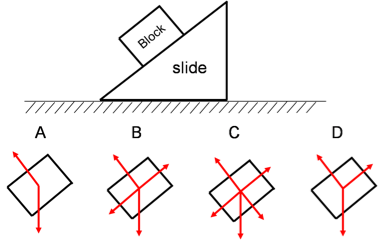
\includegraphics[scale=.4]{/Users/jgates/desktop/latex/pics/incline3.png}
%\end{floatingfigure}
 
{\bf \Large{200.}} Construct a position-vs-time graph for the motion described in the v vs t graph shown below. Assume a position of 10 meters at t = 0. Be sure to number the scale on the position axis.. 

\bigskip

%What was your original speed?  
\begin{center}
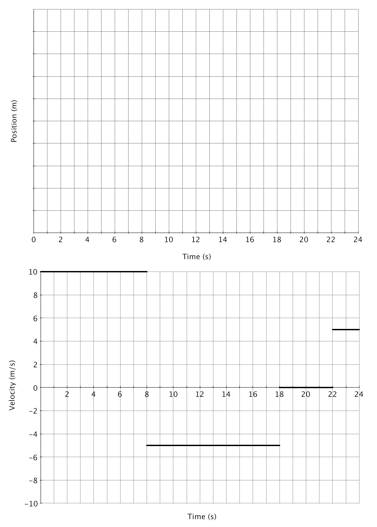
\includegraphics[scale=.77]{/Users/jgates/desktop/latex/pics/vtoxgraph1.png}
\end{center}

\bigskip 
\vspace{6mm}% Number 210
% CVPMA Algebra Units
% Flipper: x modeling given graph
% JG

% Watermark
\AddToShipoutPicture*{\BackgroundPic}

\addtocounter {ProbNum} {1}

\begin{floatingfigure}[r]{.4\textwidth}
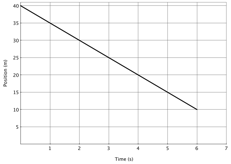
\includegraphics[scale=1]{/Users/jgates/desktop/latex/pics/flipper.png}
\end{floatingfigure}
 
{\bf \Large{210.}} Consider an x vs. t graph for Flipper (you know, the dolphin: king of the sea?).

\bigskip

Agebraically determine Flipper�s position at ${t =}$ 10 s.

%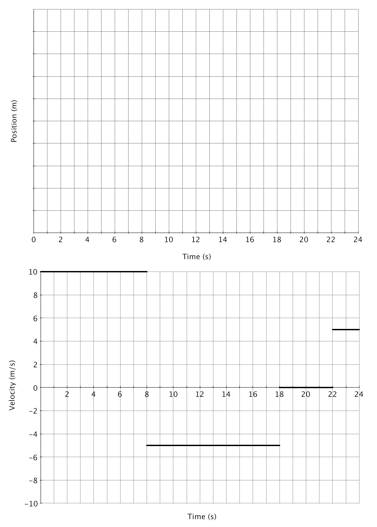
\includegraphics[scale=.77]{/Users/jgates/desktop/latex/pics/vtoxgraph1.png}

\bigskip 
\vspace{6mm}% Number 220
% CVPMG  Units
% Mongooses: avg v/speed, multiple representations
% JG

% Watermark
\AddToShipoutPicture*{\BackgroundPic}

\addtocounter {ProbNum} {1}

%\begin{floatingfigure}[r]{.4\textwidth}
%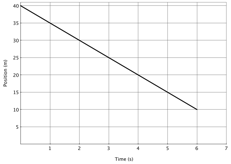
\includegraphics[scale=1]{/Users/jgates/desktop/latex/pics/flipper.png}
%\end{floatingfigure}
 
{\bf \Large{220.}} Two mongooses (mongeese?) walk around on a balance beam:

\begin{center} 
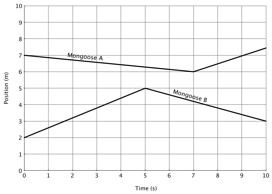
\includegraphics[scale=1]{/Users/jgates/desktop/latex/pics/mongooses.png}
\end{center}

\bigskip
Describe Mongoose A's motion in words.

\bigskip Draw a diagram describing Mongoose B's motion.

\bigskip Which mongoose has the greater average velocity?  Defend your answer.

\bigskip Which mongoose has the greater average speed?  Defend your answer.

\bigskip 
\vspace{6mm}% Number 230
% CVPMG  Units
% Dori/Danica soccer: graphical version
% JG

% Watermark
\AddToShipoutPicture*{\BackgroundPic}

\addtocounter {ProbNum} {1}

%\begin{floatingfigure}[r]{.4\textwidth}
%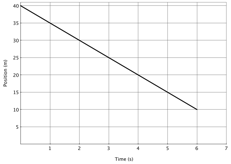
\includegraphics[scale=1]{/Users/jgates/desktop/latex/pics/flipper.png}
%\end{floatingfigure}
 
{\bf \Large{230.}} Dori's running at ${2~\tfrac{m}{s}}$ towards Tower Hill's goal line from 20 meters away when Danica lofts a ball over Dori's head.  The ball hits the ground 3 meters ahead of Dori and rolls towards the goal line at ${4~\tfrac{m}{s}}$.  

\bigskip

It takes 1.5 seconds for Dori to react to the ball; at that point, she begins running faster in order to catch up with the ball before it reaches the goal line.  
%\begin{center} 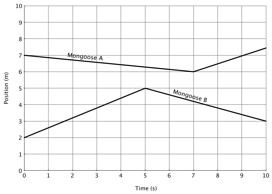
\includegraphics[scale=1]{/Users/jgates/desktop/latex/pics/mongooses.png}
%\end{center}

\bigskip

How fast does she need to run to catch up with the ball before it goes over the goal line? Use graphical problem-solving.

\bigskip 
\vspace{6mm}% Number 231
% CVPMA  Units
% Dori/Danica soccer: algebraic version
% JG

% Watermark
\AddToShipoutPicture*{\BackgroundPic}

\addtocounter {ProbNum} {1}

%\begin{floatingfigure}[r]{.4\textwidth}
%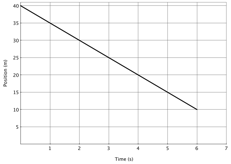
\includegraphics[scale=1]{/Users/jgates/desktop/latex/pics/flipper.png}
%\end{floatingfigure}
 
{\bf \Large{231.}} Dori's running at ${2~\tfrac{m}{s}}$ towards Tower Hill's goal line from 20 meters away when Danica lofts a ball over Dori's head.  The ball hits the ground 3 meters ahead of Dori and rolls towards the goal line at ${4~\tfrac{m}{s}}$.  

\bigskip

It takes 1.5 seconds for Dori to react to the ball; at that point, she begins running faster in order to catch up with the ball before it reaches the goal line.  
%\begin{center} 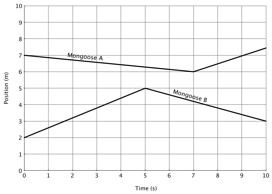
\includegraphics[scale=1]{/Users/jgates/desktop/latex/pics/mongooses.png}
%\end{center}

\bigskip

How fast does she need to run to catch up with the ball before it goes over the goal line? Use algebraic problem-solving.

\bigskip 
\vspace{6mm}% Number 240
% CVPMA Algebra  Units
% Football players running at each other: algebraic version
% JG

% Watermark
\AddToShipoutPicture*{\BackgroundPic}

\addtocounter {ProbNum} {1}

%\begin{floatingfigure}[r]{.4\textwidth}
%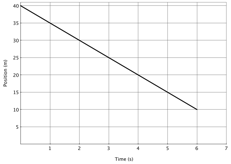
\includegraphics[scale=1]{/Users/jgates/desktop/latex/pics/flipper.png}
%\end{floatingfigure}
 
{\bf \Large{240.}} A running back carries the football down the field, running ${5.6~\tfrac{m}{s}}$.  The slower safety (running speed: ${4.5~\tfrac{m}{s}}$) runs towards him and tries to tackle him. They begin 22 meters apart and run straight at each other.  
%\begin{center} 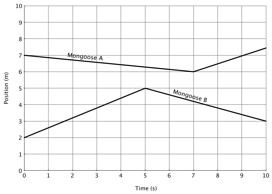
\includegraphics[scale=1]{/Users/jgates/desktop/latex/pics/mongooses.png}
%\end{center}

\bigskip

How far did the running back go before being tackled, and how much time elapsed before he was tackled? Draw a diagram and use algebraic problem solving.

 
\bigskip 
\vspace{6mm}% Number 241
% CVPMG Units
% Football players running at each other: graphical version
% JG

% Watermark
\AddToShipoutPicture*{\BackgroundPic}

\addtocounter {ProbNum} {1}

%\begin{floatingfigure}[r]{.4\textwidth}
%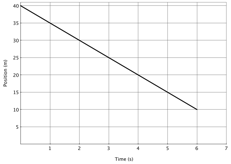
\includegraphics[scale=1]{/Users/jgates/desktop/latex/pics/flipper.png}
%\end{floatingfigure}
 
{\bf \Large{241.}} A running back carries the football down the field, running ${5.6~\tfrac{m}{s}}$.  The slower safety (running speed: ${4.5~\tfrac{m}{s}}$) runs towards him and tries to tackle him. They begin 22 meters apart and run straight at each other.  
%\begin{center} 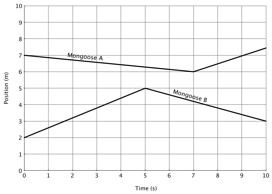
\includegraphics[scale=1]{/Users/jgates/desktop/latex/pics/mongooses.png}
%\end{center}

\bigskip

How far did the running back go before being tackled, and how much time elapsed before he was tackled? Use graphical problem solving.
 
\bigskip 
\vspace{6mm}\end{document}